\chapter{Design}
\label{ch:design}

% Budget and sources: docs/thesis/outline.md. Every claim about behaviour points at a test, a figure or a number in data/.


% Sections are written as the decisions land (docs/adr); order follows the outline, so earlier sections are
% filled in later. This one distils ADR 0002.
\section{The regime-parameterised state machine}
\label{sec:design-state-machine}

Every strand of a dispute described in chapter~\ref{ch:introduction} depends on one fact, which is where the
dispute currently stands. A clock is met by entering a state, a posting is caused by entering a state, a
notice is owed because a state was entered, and an authorization policy decides on the state the dispute is
in. The lifecycle is therefore the spine of the design, and the first decision was how to model it when four
regimes disagree about what a lifecycle contains. One option was a workflow per regime. The other, taken
here, is a single state machine whose shape is shared and whose regime decides which parts of it exist.

The shared lifecycle has fifteen states (figure~\ref{fig:state-machine}). A dispute is \emph{initiated}, an
analyst opens the \emph{investigation}, and the customer may be sent a questionnaire and answer it. The
customer may then receive money in one of three forms, which are three different states because they are
three different things in law: a \emph{provisional credit} that can be taken back, a \emph{fast refund}
that is final, and a \emph{no-questions-asked refund} of a direct debit. From there the bank may file a
chargeback, which the acquirer acknowledges, the merchant may answer with evidence, and the network rules
won or lost. A provisional credit is then either made final or reversed. Every path ends in \emph{closed},
and a closed dispute can be appealed, which reopens the investigation.

\begin{figure}[htbp]
\centering
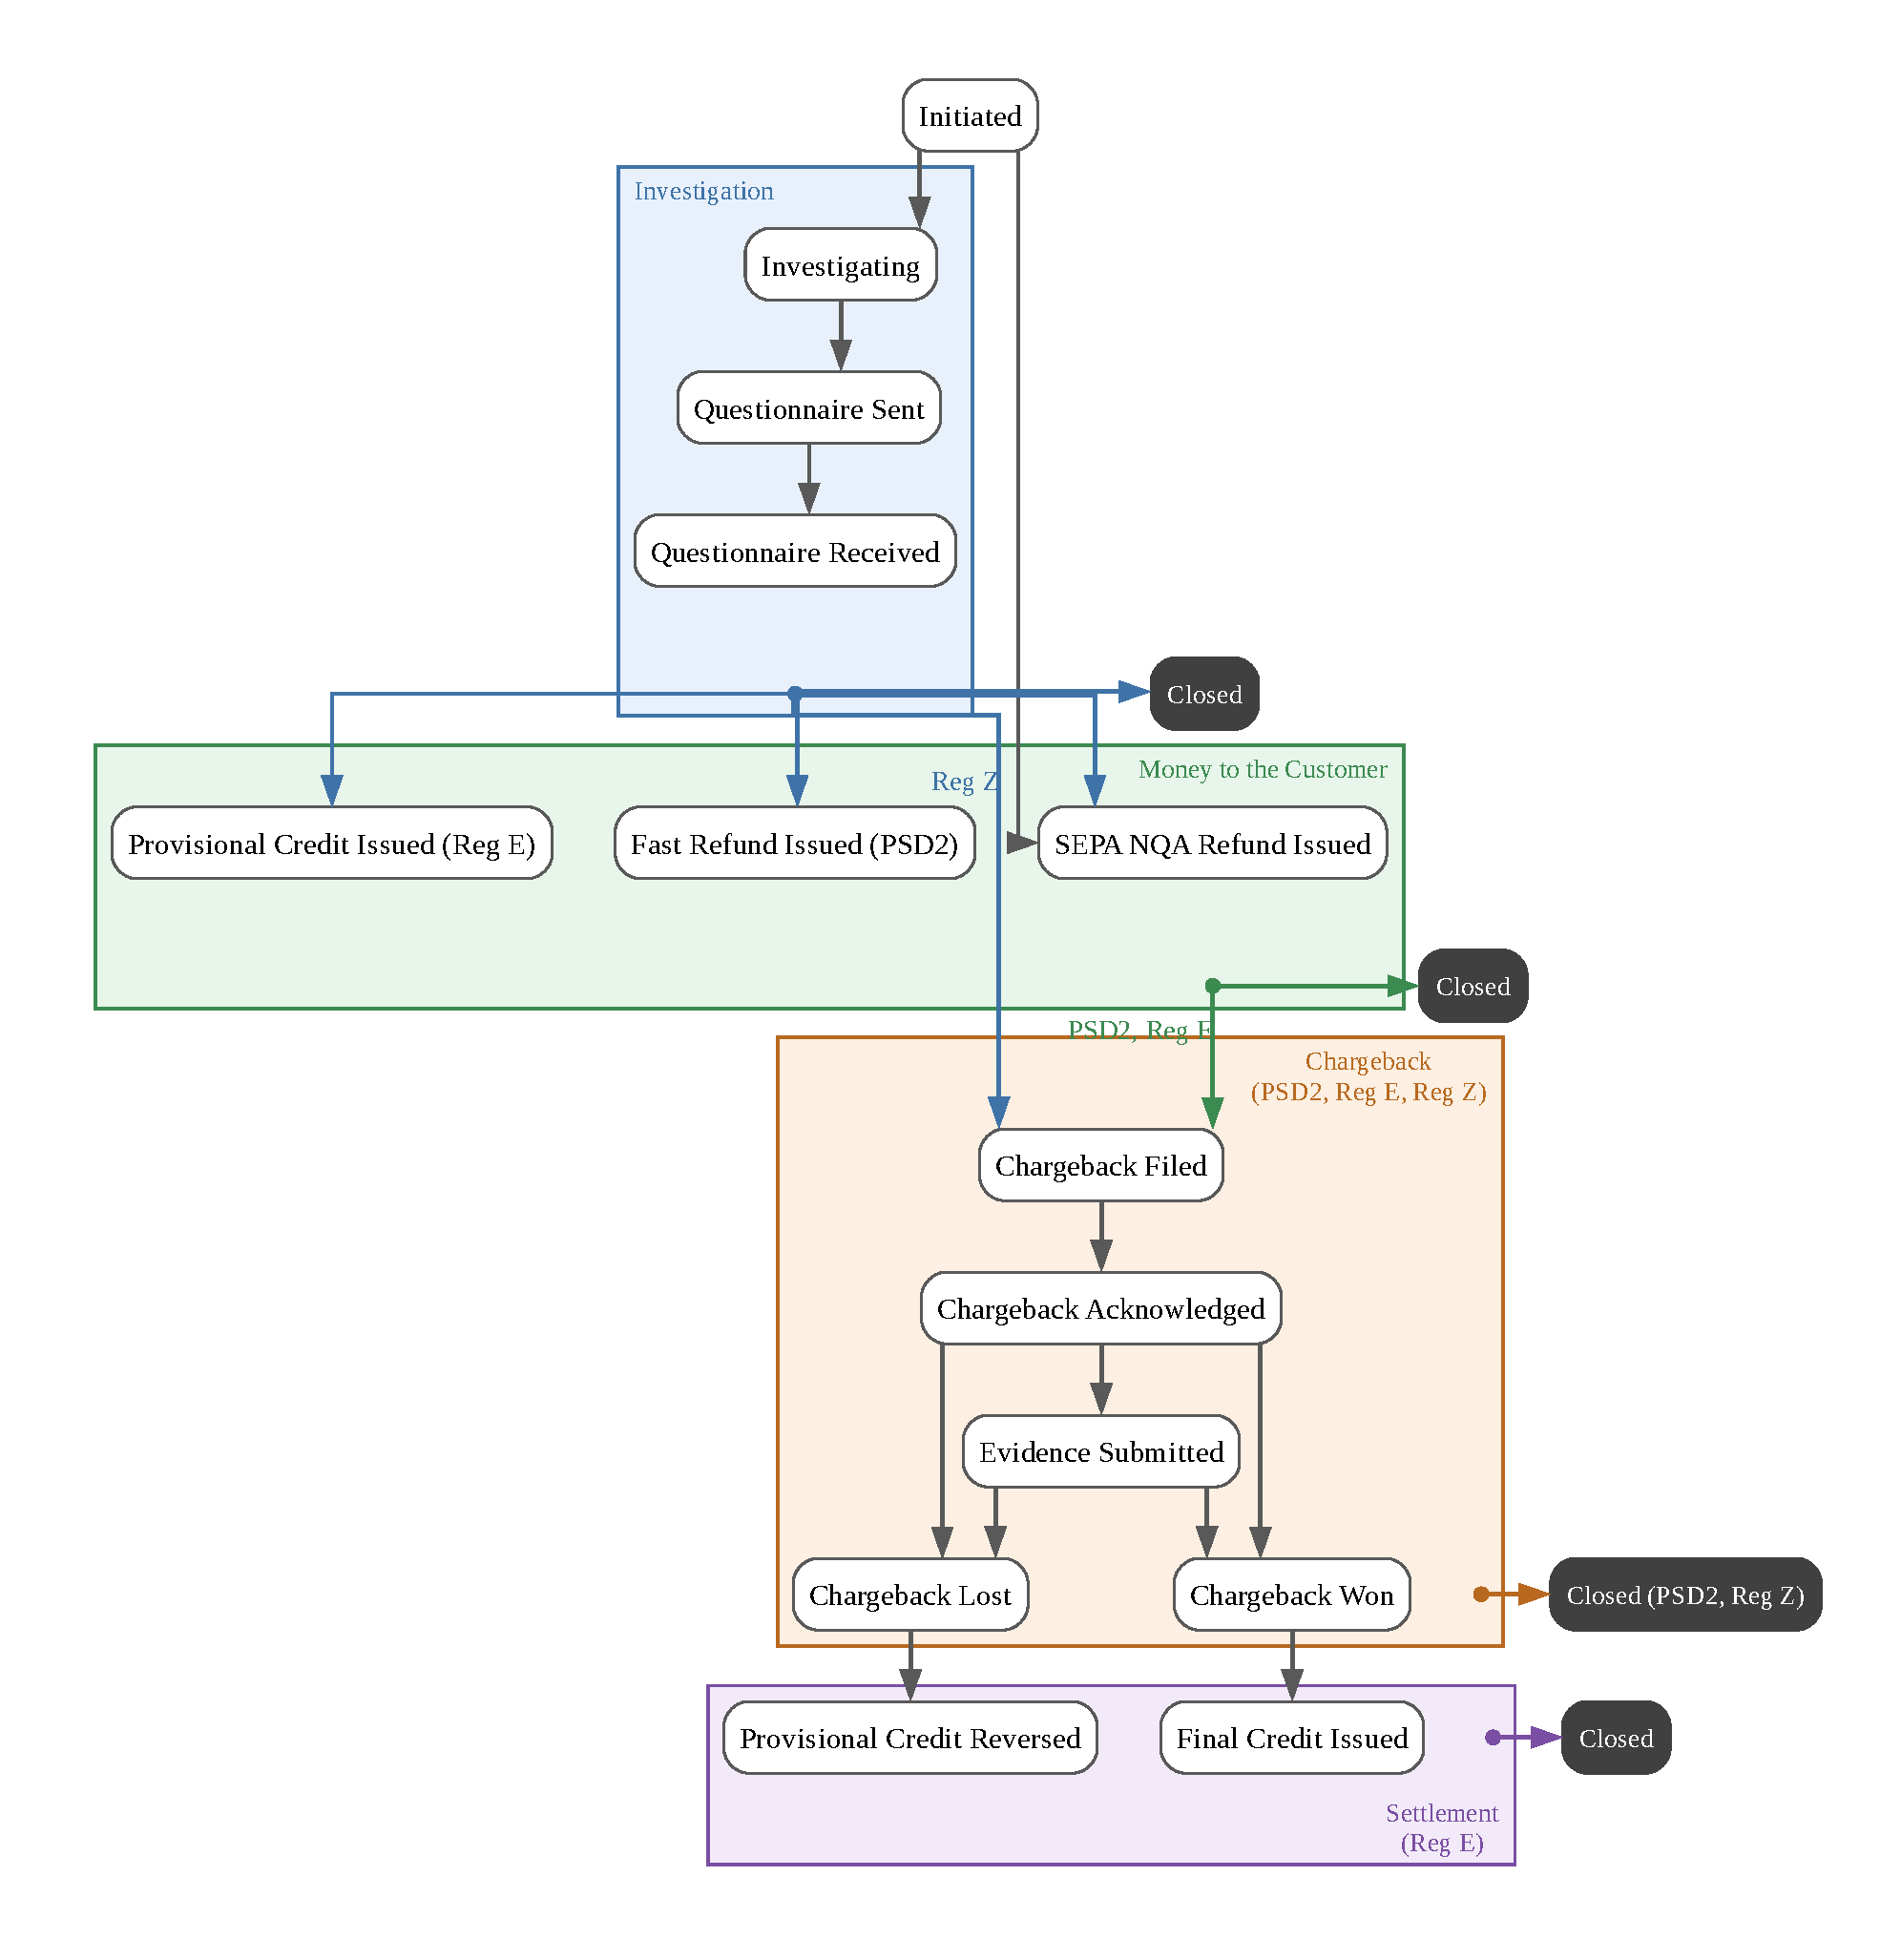
\includegraphics[width=\textwidth]{state-machine.pdf}
\caption{The dispute lifecycle under all four regimes, drawn from the transition table by a test
(\code{domain/diagram\_test.go}, \code{make thesis:figures}). Each arrow is the event that enters its target
state. Coloured boxes group the states into phases; an arrow from a dot in a phase's colour stands for the
same step taken from several of the phase's states. The dark \emph{Closed} boxes are one end state, repeated
beside each phase that can end the dispute. Names in brackets and on arrows are the regimes a state, a phase or a step is limited to (SEPA direct debit,
PSD2 card payments, Regulation~E, Regulation~Z); an unmarked arrow is open to every regime that reaches it. The appeal, from \emph{Closed} back to \emph{Investigating}
and allowed once, is not drawn.}
\label{fig:state-machine}
\end{figure}

What differs between regimes is expressed as a handful of properties of the regime's rules, never as a test
of the regime's name. The kind of money the customer receives is one: none, a no-questions-asked refund, a
fast refund or a provisional credit. Whether the regime has adjudication at all is another, and whether the
merchant may contest it a third. Whether a provisional credit exists is derived from the first. The
transition function asks these questions and nothing else. A SEPA claim can be refunded straight from
initiation, because its refund needs no investigation; a credit-card dispute under Regulation~Z files the
chargeback directly from the investigation, because there is no refund step to come first; a won chargeback
under Regulation~E cannot close until the provisional credit is made final, while under PSD2 the refund was
final all along and the dispute closes at once. The result is that the regimes reach different parts of the
same machine: six states under SEPA, eleven under PSD2, thirteen under Regulation~E and ten under
Regulation~Z. A fifth regime would be a new row of rules and its tests, not new code in the machine. The
regime itself is fixed when the dispute opens, from the transaction's rail and currency
(figure~\ref{fig:regimes}), and never changes afterwards, so a dispute cannot drift from one set of rules to
another halfway through.

The machine is a single pure function from a dispute and an event to the next dispute, written as one table
of cases rather than with a state-machine library. A library would have needed either one machine per
regime, which is the design that was rejected, or guard callbacks on shared transitions, which would hide
the table that the gates make readable. The function never changes the dispute it is given; it returns
the next one or refuses with an invalid-transition error, which the API reports as a \code{409} problem
(section~\ref{sec:design-failures}). The events a dispute currently offers are not listed anywhere: they are
found by asking the function about each event in turn. The workbench's buttons and the engine's answers
therefore cannot disagree, since they are the same computation, and a test checks it for every reachable
state of every regime. An appeal is the one transition outside the table. It is allowed only from
\emph{closed}, at most once under each regime's rules, returns the dispute to the investigation, and starts
a new resolution clock (section~\ref{sec:design-clocks}).

Its tests, from the pinned set of reachable states of each regime to a gate that fails unless a named scenario
walks every accepted transition, are reported in section~\ref{sec:eval-correctness}. Figure~\ref{fig:state-machine}
is drawn from the same table by a test that compares it with a stored copy, so changing the lifecycle fails the
build until the figure is regenerated.

\section{Regulatory clocks}
\label{sec:design-clocks}

A dispute is not only a sequence of states; it is a sequence of states that must be reached by
particular dates. The dates are where the regimes differ most visibly. PSD2 requires the payer to
be refunded ``immediately, and in any event no later than by the end of the following business
day'' \cite[art.~73(1)]{psd2} and a final reply to a complaint within fifteen business days
\cite[art.~101(2)]{psd2}; for an authorised direct debit the refund or a justification is due
within ten business days of the request \cite[art.~77(1)]{psd2}. Regulation~E requires provisional
credit within ten business days and a completed investigation within forty-five days
\cite[\S~1005.11(c)]{rege}; Regulation~Z requires a written acknowledgement within thirty days and
a resolution within two billing cycles, at most ninety days \cite[\S~1026.13(c)]{regz}. Two of the
four count business days, which depend on the jurisdiction's holidays; the others count calendar
days. An engine that treats deadlines as documentation leaves the analyst to compute them, and
leaves the institution unable to answer the auditor's first question, namely how often it met
them.

The design carries each deadline as a \emph{clock} on the regime's rules (table~\ref{fig:clocks}):
a kind, a count, a unit and the citation. There are three kinds, and each is defined by the states
that satisfy it rather than by the regime, in the same spirit as the gates of the state machine
(section~\ref{sec:design-state-machine}): the refund clock is met by entering any credit state,
the acknowledgement clock by opening the investigation, the resolution clock by closing. A clock
that can no longer be met, such as the refund clock of a dispute closed without a credit, is
voided rather than breached. An appeal restarts the resolution clock and numbers the new one by the
appeal, so a dispute's history keeps every clock it ever had.

\begin{figure}[htbp]
\centering
\small
\begin{tabular}{llrll}
\toprule
Regime & Clock & Count & Unit & Basis \\
\midrule
\code{EU\_PSD2\_CARD} & refund & 1 & business days & PSD2 art.~73(1) \\
 & resolution & 15 & business days & PSD2 art.~101(2) \\
\code{EU\_SEPA\_DIRECT\_DEBIT} & refund & 10 & business days & PSD2 art.~77(1) \\
 & resolution & 15 & business days & PSD2 art.~101(2) \\
\code{US\_REG\_E} & refund & 10 & business days & 12 CFR 1005.11(c)(1) \\
 & resolution & 45 & calendar days & 12 CFR 1005.11(c)(2) \\
\code{US\_REG\_Z} & acknowledge & 30 & calendar days & 12 CFR 1026.13(c)(1) \\
 & resolution & 90 & calendar days & 12 CFR 1026.13(c)(2) \\
\bottomrule
\end{tabular}
\caption{The clocks each regime starts when a dispute opens (\code{domain/regime.go}). Extensions the law
permits for complex cases are not modelled; see section~\ref{sec:limitations}.}
\label{fig:clocks}
\end{figure}

Two decisions follow from treating a due date as something the institution has told the customer.
First, the due time is computed once, when the dispute opens, and stored as a row alongside the
dispute under the same row-level security as everything else the tenant owns; a later change to a
rule or to a holiday calendar cannot silently move a deadline that was already communicated, and a
dispute opened before the feature existed has no clocks rather than an invented breach. Second,
the calendar is tenant data, not code: a tenant's settings name its time zone and public holidays,
entered at onboarding, and the due time is the last instant of the $n$th permitted day in that
zone; the unit tests in \code{domain/deadline\_test.go} fix weekends, holidays and the difference
between time zones.

Status is never stored. A clock is \emph{running}, \emph{met}, \emph{late} (satisfied after its
due time), \emph{breached} (open and past due) or \emph{void}, and the answer is a comparison of
three timestamps with the current time at the moment someone asks. Nothing therefore has to run
at midnight to notice a breach; the workbench's ``overdue only'' filter, the API's
\code{overdue} parameter and the overdue gauge all ask the same question of the same rows, and a
histogram of the slack at the moment each clock is satisfied turns compliance from a report into a
distribution.

% Distils ADR 0015.
\section{The banking core adapter}
\label{sec:design-core}

The ledger says what should move; a bank's core system moves it. Every tenant has its own, and
the proposal asked for a simulated one modelled on ISO 8583 field semantics. The simulator is the
least interesting part of the design. What matters is the port between the engine and whatever
core a tenant has: what is sent, what comes back, when the call is made, and what happens when
the answer is no, or never arrives.

An \emph{instruction} is one movement on the customer's account: the posting's reference, the
account, the amount and currency, whether it is a credit or a debit, and the dispute and original
transaction for the core's own records. A \emph{receipt} is the answer in the vocabulary a card
switch already uses: a retrieval reference number (field 37), a two-character response code
(field 39), whether the instruction was approved, and whether the core recognised the reference as
one it had already carried out (response code 94, duplicate transmission). Only postings that
touch the customer's account cross this port; suspense, recovery and loss are the bank's own books
and never leave the engine. Each tenant names its core in its settings and a router picks the
adapter by that name, so two tenants on one deployment can be two different banks; the two seed
tenants are configured differently on purpose, one refusing credits above a limit and one
answering slowly. The simulator behind the port in this build speaks the message types and fields a real
switch would, remembers what it has seen, and can be told per tenant to decline, to refuse debits
on named accounts, to be slow or to be down (\code{infrastructure/mockcore}).

The decision that shapes everything else is \emph{when} to call. The engine calls the core inside
the transition's own database transaction, with a bounded timeout, and treats the answer as part
of the transition. A decline rolls the transition back: the response is a 422 problem carrying the
core's response code, and the dispute has no new event and no new posting. Silence rolls it back
too, as a 503 the client is told to repeat with the same idempotency key. Because the transition
was never written, the repeat computes the same event sequence and therefore the same posting
reference; a core that did move the money before its answer was lost recognises the reference
and answers duplicate instead of paying twice, and the engine records that receipt as the
approval it is. The alternative, an outbox with a reconciliation job, buys the engine freedom from
the core's latency at the price of a window in which the dispute says the customer was refunded
and the core disagrees. For a system whose one job is to be right about that, the lock is the
cheaper price. Its cost is real: a slow core slows that dispute, though no other, and the test
\code{TestARetryAfterSilenceIsADuplicateNotADoublePayment} is the promise that the retry story
holds.

% Distils ADR 0014.
\section{The ledger}
\label{sec:design-ledger}

Three of the four regimes move the customer's money before anyone knows who was right. Under
Regulation~E the bank posts a provisional credit it may later take back; under PSD2 it refunds at
once and absorbs the loss unless a chargeback recovers it; under SEPA Core it refunds and the
scheme recovers the amount from the creditor's bank. The original design (appendix, wiki extract)
imagined a provisional-credit engine and a final-credit engine as separate components. Both
disappear into one small ledger once the question is put correctly: not ``what kind of credit is
this?'' but ``where is the money now?''

The ledger has four accounts from the issuer's point of view (figure~\ref{fig:ledger}): the
customer's account, a suspense account holding what the bank has advanced and not yet cleared, and
recovery and loss, which clear it. Every movement is a double-entry posting, and every posting is
caused by a transition: entering a credit state debits suspense and credits the customer; a
reversal does the opposite; a won chargeback recovers; a lost chargeback writes off, unless the
regime has provisional credit, in which case the reversal that follows takes the advance back from
the customer instead; and closing settles whatever remains, recovered or written off, by the
analyst's word or the regime's default. As with the state machine and the clocks, nothing here
tests the regime's name: the postings follow from the state entered and two properties of the
rules.

\begin{figure}[htbp]
\centering
\small
\begin{tabular}{L{5.5cm}L{4.1cm}L{2.4cm}L{1.6cm}}
\toprule
State entered & Posting & Debit & Credit \\
\midrule
any credit state & credit (disputed less liability) & suspense & customer \\
\code{PROVISIONAL\_CREDIT\_REVERSED} & reversal (outstanding) & customer & suspense \\
\code{CHARGEBACK\_WON} & recovery (outstanding) & recovery & suspense \\
\code{CHARGEBACK\_LOST}, no provisional credit & write-off (outstanding) & loss & suspense \\
\code{CLOSED}, outstanding & settlement, recovered or written off & recovery or loss & suspense \\
\bottomrule
\end{tabular}
\caption{Postings caused by entering a state (\code{domain/ledger.go}). ``Outstanding'' is the dispute's suspense
balance before the transition; a posting of zero is not written.}
\label{fig:ledger}
\end{figure}

The property that matters is that suspense is zero when a dispute closes: whatever the bank
advanced was taken back, recovered or written off, and nothing is left in limbo. It is not
enforced by a check at close. It holds by construction, and the test suite proves it the way the
state machine's dead-end freedom is proved (section~\ref{sec:design-state-machine}): a test
enumerates every path from \code{INITIATED} to \code{CLOSED} under every regime, forty-three at
the time of writing, replays each through the posting rules with each settlement choice, and
asserts a zero balance and a customer who never ends up net debited
(\code{TestSuspenseBalancesOnEveryPath}). A regime or state added later that breaks the invariant
fails the build rather than a reconciliation months on.

The amount credited is the disputed amount less a liability the analyst may assign to the
customer, capped by the regime (figure~\ref{fig:regimes}). The liability
travels in the refund event's payload, as does the settlement choice on close; both are validated
against the regime before the transition is written, and a refusal is a 422 problem naming the
field, after which the dispute is exactly as it was: no event, no posting. Postings themselves are
rows under the same row-level security as the dispute, append-only at the database like the event
log, each keyed to the event that caused it and carrying a reference unique within the tenant.
That reference is the idempotency key the banking core adapter (section~\ref{sec:design-core})
uses, so an instruction repeated after a timeout cannot move money twice.

% Distils ADR 0018.
\section{Fraud scoring}
\label{sec:design-fraud}

The proposal ended with a fraud-scoring engine, marked from the outset as the first thing to
cut if time ran short. It survived in a deliberately modest form, and the form is the point.
A learned model needs labelled outcomes the project does not have and an evaluation the thesis
cannot honestly perform; and in a process where the customer has a right to know why they were
refused, a score nobody can explain is a liability rather than an asset. The engine therefore
scores with fixed, readable rules. Seven signals, each with a fixed weight and a fixed way of
earning points, each reporting a sentence that says why it scored what it did, whether or not it
fired: how many other disputes the account raised in twelve months, how many it lost at the
network, how long after the transaction the dispute came, whether the merchant's category is one
where disputes concentrate, the amount, the account's age, and the contradictions in the
questionnaire (section~\ref{sec:design-questionnaire}). The score is the sum, and three
thresholds make it a tier.

Two decisions keep the score honest. It is assessed when the dispute opens, from what the engine
already knows, and assessed again when the questionnaire arrives, because that is when the
consistency signal becomes known; every assessment is kept, so the analyst sees the picture change
rather than a number that was always there. And its only teeth are a hold: a credit on a dispute
whose latest tier is high is refused until the analyst records why it should go out anyway, and
that justification is stored on the event with everything else. The score never denies a dispute,
never moves a state and never speaks to the customer. It orders the queue and it makes a human
write a sentence before money leaves on a case the rules distrust, which is what a scoring
engine in a regulated process can responsibly do. The weights are judgement, not fitted to data;
chapter~\ref{ch:evaluation} says so and treats them as a demonstration of the mechanism rather
than a claim about fraud.

% Distils ADR 0016.
\section{The questionnaire}
\label{sec:design-questionnaire}

Two events, \code{SEND\_QUESTIONNAIRE} and \code{RECEIVE\_QUESTIONNAIRE}, have been in the state
machine from the start; until this point nothing stood behind them. The questionnaire is where the
customer's claim becomes structured data, and structure is what the investigation and the fraud
scoring (section~\ref{sec:design-fraud}) consume. Three decisions give it its shape.

First, a dispute has a \emph{reason} from the moment it opens: unauthorised transaction, goods or
services not received, duplicate charge, or an amount that differs from what was agreed. The
reason is immutable and selects the question set; the tenant systems that already open disputes
without one get the unauthorised set, which is what they were implicitly claiming. Second, the
questions are \emph{snapshotted} onto the dispute when sent. Question sets are code, and code
changes; an answer must always be readable against the exact question the customer saw, so the
sent set is stored with the dispute and a later change to the code changes nothing already sent.
Third, answers are \emph{typed facts}, not text: yes or no, a date, an amount, or free text, each
validated against the snapshot when received, with every problem reported at once and per
question, and the transition refused as a whole when any is wrong. A questionnaire answered with
``perhaps'' to a yes-or-no question is not partly received.

The immediate consumer is the analyst, who sees the answers beside the actions; the panel that
shows them is the same one that records them, since in this engine the analyst enters what the
customer said. The second consumer is the contradiction check the domain runs over the answers:
a customer who recognises the merchant, held the card, and shared it with nobody is claiming an
unauthorised payment that the answers do not support. These are sentences an analyst can act on,
and in section~\ref{sec:design-fraud} they become one of the signals a risk score is built from.

% Distils ADR 0006 and ADR 0012.
\section{The contract and its error taxonomy}
\label{sec:design-failures}

The engine is written in Go and the workbench in TypeScript, and the two share no code at runtime. What they must
share is an agreement: which requests exist, what their bodies look like, which rules a field obeys, and what each
failure means. An agreement kept in two languages by hand drifts, so the design keeps it in one place. A single
OpenAPI document is the contract, and nothing about the HTTP surface is decided anywhere else. The server's
interface is generated from it, so a route that is not in the document does not compile, and every request is
validated against the document before any handler sees it. The client's types, its request functions and the
schemas its forms validate with are generated from the same document. The generated code is committed, and the
build fails if regenerating it would change anything, so the document and both sides cannot disagree for longer
than one failed check. Only structural rules travel this way, such as a required field or the format of an
identifier; whether a transaction exists or a transition is allowed remains the server's to decide.

Failures get the same treatment, because a client that has to read error messages to decide what to do will
eventually get it wrong. Every failure the engine produces is created with a \emph{kind} and a \emph{code}. The kind
is one of nine classes, from an invalid request to an unavailable dependency, and decides the HTTP status, whether
the failure is logged and whether repeating the request can help. The code is a stable, machine-readable name such
as \code{invalid-transition}, one of 28 the contract lists. A handler never chooses a status: one table maps kind to
status for the whole service. The response is a problem document in the standard format for HTTP APIs
\cite{rfc9457}, extended with the code, whether the request is worth retrying and after how long, a reference to
the request, and, for a validation failure, one entry per field pointing at the field in the body
(figure~\ref{fig:problem}). Two codes carry what a client needs to recover: a refused transition lists the events
the dispute does allow, and a rate limit says when to come back.

\begin{figure}[htbp]
\begin{lstlisting}
HTTP/1.1 409 Conflict
Content-Type: application/problem+json

{"type": "urn:dispute-engine:error:invalid-transition",
 "title": "The request conflicts with the current state",
 "status": 409,
 "detail": "this action is not allowed in the dispute's current state",
 "instance": "/disputes/01a15551-c90d-7c55-bfe5-368b97457880/events",
 "code": "invalid-transition",
 "retryable": false,
 "requestId": "ab1de00df2f8ba20",
 "allowedEvents": ["OPEN_INVESTIGATION"]}
\end{lstlisting}
\caption{The response to an analyst who tries to win the chargeback of a PSD2 dispute that has only just opened,
captured from the service's handler.}
\label{fig:problem}
\end{figure}

Everything in a problem document is written to be shown to the person who caused it. The diagnostic context that
an engineer needs, such as the regime and the state the dispute was in, is attached to the error for the logs and
the trace and never reaches the body; a test checks that it does not leak. A failure nobody classified becomes a
generic internal error whose only detail is the request reference, under which the logs and the trace hold the
cause. The list of codes is kept in two places, the contract and the Go code that emits them, and a test fails if
the two ever differ.

The workbench classifies every response once into a closed set of ten failure kinds, nine from the server's
codes and one, an unreachable server, that only a client can observe; the table from code to kind must cover every
code in the contract, which the compiler checks, and a page decides what to show from the kind, never from a
message.

% Distils ADR 0008, 0009, 0010 and 0020.
\section{Multi-tenancy with row-level security}
\label{sec:design-tenancy}

The engine serves several institutions from one deployment. They share the regulatory logic and the process;
they must never share data, and the design must not depend on every query remembering that. Three layouts were
considered: a database per tenant, a schema per tenant, and one schema in which every row names its tenant. The
first two isolate well but multiply everything an operator has to run, from migrations to dashboards, by the
number of customers. The third keeps one of everything, and is only safe if isolation is enforced somewhere a
forgotten filter cannot reach. The design takes the third and puts the enforcement in the database, with
PostgreSQL's row-level security \cite{pgrls}.

Every business table carries the tenant's identifier, and every one has the same policy: a row is visible, and
may be written, only when its tenant is the one bound to the current transaction (figure~\ref{fig:rls}). The
service binds the tenant at the start of each transaction from the authenticated caller, never from anything the
client sends, and binds it for that transaction only, so a pooled connection cannot carry one tenant's identity
into another tenant's request. When nothing is bound the setting is empty and the policy matches no rows, so
every mistake in this area fails closed; the store also refuses to open a transaction at all without a tenant.
The service runs as a database role that is subject to the policies, while the schema's owner, which runs
migrations, is not. The two things the service legitimately needs across tenants, a count of disputes by state
for the dashboards and the purge of expired idempotency keys, are provided by the owner as a view and a function
rather than by giving the service broader access. Idempotency keys are themselves scoped by tenant, because clients
choose them and two tenants may choose the same one.

\begin{figure}[htbp]
\begin{lstlisting}[language=SQL]
CREATE FUNCTION current_tenant_id() RETURNS uuid LANGUAGE sql STABLE AS $$
    SELECT NULLIF(current_setting('app.tenant_id', true), '')::uuid
$$;
CREATE POLICY tenant_isolation ON disputes
    USING (tenant_id = current_tenant_id())
    WITH CHECK (tenant_id = current_tenant_id());

-- at the start of every transaction (Store.WithTx), local to that transaction
SELECT set_config('app.tenant_id', $1, true);
\end{lstlisting}
\caption{The tenant policy, here on \code{disputes} (\code{migrations/0003\_tenants.sql}), and the binding the
store makes before any query. An unbound setting yields \code{NULL}, which matches no rows.}
\label{fig:rls}
\end{figure}

The tenant therefore has to come from the credential, and there are two kinds of caller with different needs.
A tenant's own systems, such as the online bank that opens disputes, run unattended and expect a credential they
can store: they present a \emph{tenant key}, a random secret shown once when it is issued and kept only as a hash,
which names its tenant and can be revoked on its own. Analysts are people, and sign in through an identity provider
\cite{oidc} in which every tenant has its own realm, so each institution's users and sign-in rules are
separate from every other's at the level of the identity system, not only by a field in a token. The tenant's short name in the address of the workbench chooses the realm before
anyone signs in. The engine verifies an analyst's token itself: the issuer of the token decides the tenant, an
issuer that no tenant owns is refused, and a tenant claim inside the token that disagrees with its issuer is
refused as a sign of a misconfigured realm. Both kinds of credential end in the same context, a tenant and a
principal, and everything below that point is shared.

The browser never holds either credential; how the workbench keeps an analyst's tokens on its server is
described in section~\ref{sec:impl-sessions}. The price of the design is that
every new table needs its tenant column, its policy and its grants, and a table that lacks them fails a test of the
service role's privileges before it can be released. The isolation it buys is tested against the database role
the service actually uses, as chapter~\ref{ch:evaluation} reports (section~\ref{sec:eval-isolation}).

% Distils ADR 0026.
\section{Authorization}
\label{sec:design-authorization}

Row-level security answers which tenant a row belongs to; it says nothing about who inside a
tenant may do what. Until this point the answer was everyone: any analyst or tenant key could
apply any event, including the ones that move money, and the actor written on each event was
whatever the request claimed. An issuer's own operations run on the opposite assumptions. Work
belongs to teams, seniority bounds the amounts a person may settle alone, and the person who
investigated a claim does not also pay it out. The engine therefore decides every operation that
changes a dispute or the tenant with one policy engine, over one notion of the caller.

The caller is a \emph{principal}, the same shape for both credentials of section~\ref{sec:design-tenancy}:
an analyst, named by the subject of their token and carrying whether their realm made them a
tenant administrator, or a tenant key, named by its identifier. The event actor is always this
principal and never a field of the request, so the audit trail records who acted rather than who
claimed to. That change is what makes the rest of the model meaningful, since a rule about who
opened an investigation is only as good as the record of who did.

Policies are written in Cedar \cite{cedar2024}, evaluated inside the service. Cedar was chosen over
a general-purpose policy language and over a purpose-built one for three properties the argument
depends on. It denies by default. It resolves conflicts in one fixed way: any policy that forbids
an action overrides every policy that permits it. And its semantics are specified formally, with
a reference implementation that can check a policy set against a schema before it is ever
evaluated. The engine splits its policies along that first property. \emph{Guardrails} are Cedar
in the binary that no tenant can change, written as prohibitions: whoever opened the
investigation never issues its final credit, only a lead of a dispute's team may move it
elsewhere, tenant administration follows the realm role and nothing else, and a tenant key never
writes to a customer. \emph{Grants} are data, one row per team, role and action, optionally bounded
by an amount, compiled into permissions that can reach only their own team's disputes. A grant
that cannot be expressed safely is dropped rather than escaped, so a malformed row can only take a
permission away. Because a prohibition always wins, no combination of grants can open what a
guardrail closes; that is the property that later lets tenants edit their own grants without the
engine trusting what they write.

The decision is made where the facts are committed: inside the request's transaction, after the
dispute is loaded and before the state machine runs. What the policies see is the dispute's team,
amount, rail and state, and who opened its investigation, taken from the event log rather than
from the request. A refusal names the policy that decided it, and an allowed event records the
policies that allowed it, so the log answers why a credit was permitted as well as who issued it.
The actions a dispute offers are the ones the state machine would accept and the caller may take,
so the workbench never shows a button that would be refused. Two smaller decisions close gaps the
model would otherwise leave: an idempotency key belongs to the principal that used it, so a
replayed response is never handed to someone the engine did not authorize, and the service
refuses to start if any operation in its contract has not been classified as public, internal,
open to any caller of the tenant, or decided by the engine.

% Distils ADR 0027.
\subsection{Teams, grants and a second line}
\label{sec:design-teams}

A dispute belongs to one team, chosen when it opens by the first routing rule that matches its
rail, reason and amount, and otherwise by the tenant's default team. Inside a team a person holds
one rung of a fixed ladder, junior, senior or lead, and the ladder is expressed in Cedar's own
hierarchy: a lead is a member of senior, which is a member of junior, so a grant to juniors reaches
every rung above without any role logic in code. Teams, memberships, grants and routing are rows,
and any change to them advances a version that invalidates the tenant's compiled policies on the
next request. The rows are what a tenant administrator will one day edit, and the argument of the
previous paragraphs is what makes that safe: grants compile only to permissions bounded by their
team, while everything that must always hold is a prohibition in the binary. Generated sets of
arbitrary grants confirm the three properties that matter, that no set lets an investigator pay
out their own dispute, reaches a dispute outside the caller's teams, or administers the tenant;
removing the separation-of-duties rule makes the first of them fail, which is the evidence the
property can fail at all.

Team scope is enforced twice. Beside the policy decision, row-level security narrows every read to
the caller's teams, so a check forgotten in a handler still cannot show one team another's work,
and a dispute outside those teams answers as if it did not exist. The policies are restrictive
rather than permissive, a distinction with teeth: PostgreSQL combines permissive policies with
\emph{or}, so a permissive team policy beside tenant isolation would have widened what a caller
sees rather than narrowed it \cite{pgrls}. The two lines disagree in one place by design.
Reassigning a dispute to a team the lead is not in cannot pass a row policy, because an update's
new row must also be readable by the caller; that single move therefore runs as the owner,
bounded to the caller's tenant, current membership and the version they read, after the policy
engine has allowed it. What this costs per request is measured in section~\ref{sec:eval-latency}: extra round trips
rather than policy evaluation, a price of deciding inside the request's transaction on committed facts.

% Distils ADR 0017.
\section{Communications}
\label{sec:design-communications}

A dispute is a conversation with the customer as much as a sequence of states, and the regimes
say when the bank must speak: Regulation~Z wants a written acknowledgement within thirty days
\cite[\S~1026.13(c)(1)]{regz}; Regulation~E wants the customer told of a provisional credit
\cite[\S~1005.11(c)(2)(iv)]{rege}, told the date and amount of a reversal before it happens
\cite[\S~1005.11(d)(2)]{rege}, and told the outcome with the right to see the documents relied on
\cite[\S~1005.11(d)(1)]{rege}. What the bank owes is therefore domain knowledge, and the engine
keeps it where it keeps the rest: a function from the state entered to the notices it triggers,
and a second from the regime's rules to the channels, email always and a printable letter as well
where the regime's notices must be in writing. As with the clocks and the ledger, the gate is a
property of the rules, never a regime's name.

The design question is again \emph{when}. Sending is a side effect that can fail, and a transition
must not be undone because a mail relay was down; but a notice that is owed must not be lost
because the process died between the commit and the send. The engine composes the notice inside
the transition, from facts it already holds (the account, the original transaction, the running
clocks, the ledger, the questionnaire), as structured paragraphs with the provision each one
satisfies, and stores it as a row in the same transaction. A letter is thereby complete the moment
it exists; the workbench lays it out on a printable page from the paragraphs, so no markup is ever
trusted. An email is an entry in an outbox, which a dispatcher drains after every commit and on a timer,
so a notice survives a crash between the commit and the send. The trade is the usual one for an
outbox: delivery is at-least-once, so a relay that accepted a message but failed to say so may
receive it twice, whereas a letter, being a row, cannot be duplicated.

Analysts also write on their own initiative, to ask for documents or to report where a case
stands, and the same machinery serves them through a small addition (ADR~0019). Their emails are
templates kept as data, each a form and a set of paragraphs in a deliberately tiny substitution
language: placeholders for the analyst's fields and for facts the engine knows, sections that appear
only when a field has a value, list-valued fields that become bullet lines. The API returns each
template with the facts already filled and the fields left as placeholders, so the browser can
preview the message live by the same substitution while the analyst types, and the server renders
the final message from the same paragraphs on send. Preview and letter therefore cannot disagree,
the analyst's email is a notice row like any other with its author recorded, and a machine
credential cannot compose one at all.

Two smaller consequences follow. The acknowledgement clock of section~\ref{sec:design-clocks} is
met by the acknowledgement notice, not by any state, because the acknowledgement is what the
regulation asks for. And the customer's file becomes complete and auditable from the dispute alone:
every paragraph ever sent, to which address, by which channel, and whether it went. Golden files pin the paragraphs of
every kind of notice under each regime, so a change in what a customer reads is a reviewed diff.
